\documentclass{article}

\usepackage{amsmath}
\usepackage{amssymb}
\usepackage{bm}
\usepackage{color}
\usepackage{CJKutf8}
\usepackage{color}
\usepackage{enumitem}
\usepackage{graphicx}
\usepackage{indentfirst}
\usepackage{listings}
\usepackage{mathdots}
\usepackage{tikz}
\usepackage{wasysym}
\usepackage{xcolor}

\setlength{\parindent}{2em}

\usetikzlibrary{shapes,arrows, automata}

\allowdisplaybreaks

\newcommand{\hytt}[1]{\texttt{\hyphenchar\font=\defaulthyphenchar #1}}
\hyphenation{read-Sym-bol re-ad-Space-Tab-New-line str-Tab}

\definecolor{mygreen}{rgb}{0,0.6,0}
\definecolor{mygray}{rgb}{0.5,0.5,0.5}
\definecolor{mymauve}{rgb}{0.58,0,0.82}
%\footnotesize
\lstset{ %
  backgroundcolor=\color{white},   % choose the background color; you must add \usepackage{color} or \usepackage{xcolor}
  basicstyle=\ttfamily,            % the size of the fonts that are used for the code
  breakatwhitespace=false,         % sets if automatic breaks should only happen at whitespace
  breaklines=true,                 % sets automatic line breaking
  captionpos=b,                    % sets the caption-position to bottom
  commentstyle=\ttfamily\color{mygreen},    
                                   % comment style
  deletekeywords={},               % if you want to delete keywords from the given language
  escapeinside={},                 % if you want to add LaTeX within your code
  extendedchars=true,              % lets you use non-ASCII characters; for 8-bits encodings only, does not work with UTF-8
  frame=single,                    % adds a frame around the code
  keepspaces=true,                 % keeps spaces in text, useful for keeping indentation of code (possibly needs columns=flexible)
  keywordstyle=\color{blue},       % keyword style
  language=VHDL,                    % the language of the code
  morekeywords={},                 % if you want to add more keywords to the set
  numbers=left,                    % where to put the line-numbers; possible values are (none, left, right)
  numbersep=5pt,                   % how far the line-numbers are from the code
  numberstyle=\tiny\color{mygray}, % the style that is used for the line-numbers
  rulecolor=\color{black},         % if not set, the frame-color may be changed on line-breaks within not-black text (e.g. comments (green here))
  showspaces=false,                % show spaces everywhere adding particular underscores; it overrides 'showstringspaces'
  showstringspaces=false,          % underline spaces within strings only
  showtabs=false,                  % show tabs within strings adding particular underscores
  stepnumber=1,                    % the step between two line-numbers. If it's 1, each line will be numbered
  stringstyle=\color{mymauve},     % string literal style
  tabsize=2,                       % sets default tabsize to 2 spaces
  title=\lstname                   % show the filename of files included with \lstinputlisting; also try caption instead of title
}

\begin{document}
\begin{CJK*}{UTF8}{gbsn}
\CJKtilde

\title{实验十\ 简易数字钟设计实验}

\author{计算机1202 张艺瀚\\学号:20123852}
\maketitle

\section{实验目的}
\begin{enumerate}
\item 学习掌握数字系统综合设计方法。
\item 学习掌握层次设计方法。
\item 学习掌握设计下载方法。
\item 学习掌握实验系统使用方法。
\end{enumerate}

\section{实验原理}
数字钟是对输入时基秒脉冲进行计数,依次输出秒数值、分数值、小时数值,从而确定时钟时间,其原理框图如图~\ref{fig: principle}所示。

\begin{center}
\begin{figure}[h!]
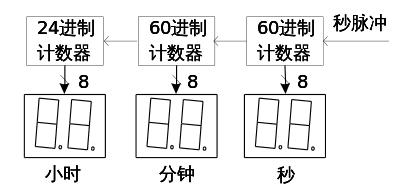
\includegraphics[width=\textwidth]{principle.jpg}
\caption{简易数字钟原理图}
\label{fig: principle}
\end{figure}
\end{center}

实际的数字钟设计中还需要增加年月日的功能,这里框图中也省略了校时功能的结构。

\section{实验内容}
\begin{enumerate}
\item 选择XC2S200PQ208器件建立一个新的 工程。
\item 在上述工程中,采用VHDL语言的方法设计上述简易数字钟。
\item 参考实验系统使用说明,按下列要求锁定引脚。秒、分钟、小时由实验系统的J1、J2输出,显示输出的时分秒间隔一位数码管。时钟输入由J7的1脚输入。
\item 下载编程并验证设计结果。
\end{enumerate}

\section{实验设备}
\begin{enumerate}
\item 清华同方PⅣ 2.4G/256M60G
\item ISE 6.2i—Windows软件系统
\item 多功能EDA实验系统(V型)
\end{enumerate}

%\section{实验步骤}

\section{实验程序}
数字钟代码清单如下(代码清单~\ref{lst: clocklst} )
\begin{center}
\begin{lstlisting}[caption = {数字钟代码清单}, label = {lst: clocklst}]
library IEEE;
use IEEE.STD_LOGIC_1164.ALL;
use IEEE.STD_LOGIC_ARITH.ALL;
use IEEE.STD_LOGIC_UNSIGNED.ALL;

--  Uncomment the following lines to use the declarations that are
--  provided for instantiating Xilinx primitive components.
--library UNISIM;
--use UNISIM.VComponents.all;

entity second is
    Port ( clk : in std_logic;
           clr1 : in std_logic;
           clr2 : in std_logic;
           en : in std_logic;
           s1 : out std_logic_vector(3 downto 0);
           s2 : out std_logic_vector(3 downto 0);
           m1 : out std_logic_vector(3 downto 0);
           m2 : out std_logic_vector(3 downto 0);
           h1 : out std_logic_vector(3 downto 0);
           h2 : out std_logic_vector(3 downto 0));
end second;

architecture Behavioral of second is
  signal cq0,cq1,cq2,cq3,cq4,cq5:std_logic_vector(3 downto 0);
begin
process(clk,clr1,clr2)				
begin
   if( clr1='0' )then
     cq0<="1000"; cq1<="0101";
     cq2<="1000"; cq3<="0101";
     cq4<="1001"; cq5<="0001";
   elsif( clr2='0' )then
     cq0<="1000"; cq1<="0101";
     cq2<="1000"; cq3<="0101";
     cq4<="0011"; cq5<="0010";
   elsif clk='1' and clk'event then				
     if(en='1') then
       if cq0="1001" and cq1="0101" then
	     cq0<="0000"; cq1<="0000"; 
	     if cq2="1001" and cq3="0101" then
		   cq2<="0000"; cq3<="0000";
		   if cq4="0011" and cq5="0010" then
		      cq4<="0000"; cq5<="0000";
		   elsif cq4="1001" then
			 cq4<="0000"; cq5<=cq5+1;
		   else  
			 cq4<=cq4+1;
		   end if;
	     elsif(cq2="1001") then 
		   cq2<="0000"; cq3<=cq3+1;
	     else 
		   cq2<=cq2+1;
	     end if;
	  elsif(cq0="1001")   then
	     cq1<=cq1+1; cq0<="0000";
	  else 
          cq0<=cq0+1;
	  end if;
     end if;
   end if;
end process;
s1<=cq0;
s2<=cq1;
m1<=cq2;
m2<=cq3;
h1<=cq4;
h2<=cq5;

end Behavioral;
\end{lstlisting}
\end{center}

\section{仿真结果}
\begin{center}
\begin{figure}[h!]
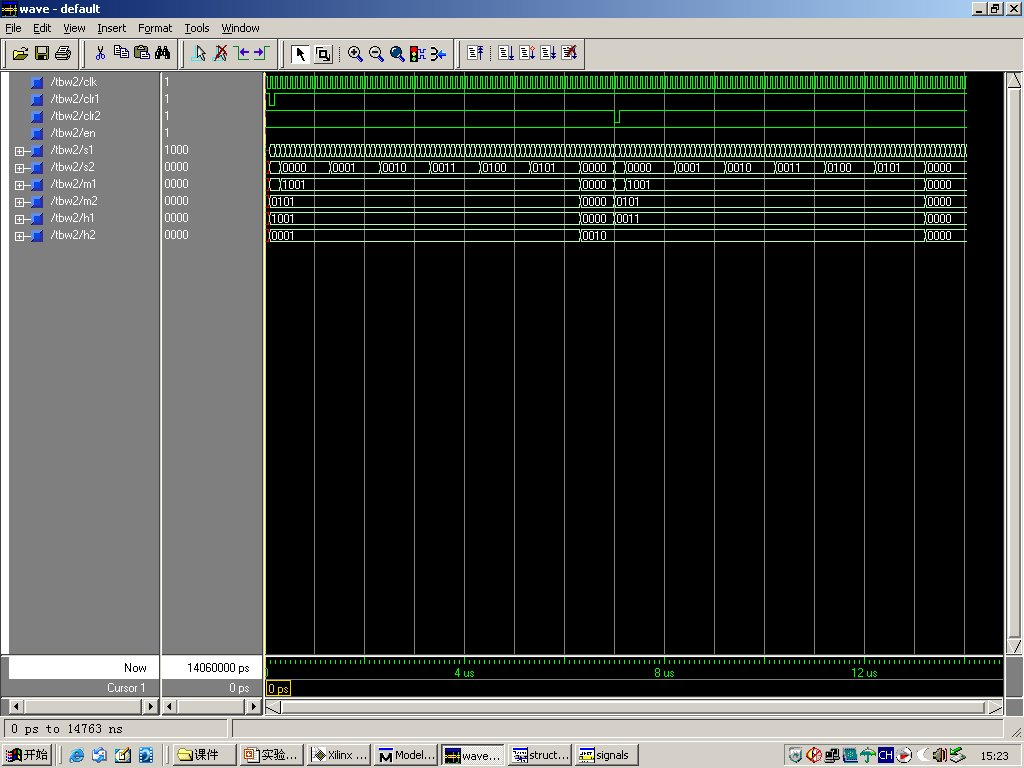
\includegraphics[width=\textwidth]{tbw.jpg}
\caption{数字钟仿真波形图}
\label{fig: cfig}
\end{figure}
\end{center}

\end{CJK*}
\end{document}
